

\tikzset{every picture/.style={line width=0.75pt}} %set default line width to 0.75pt        

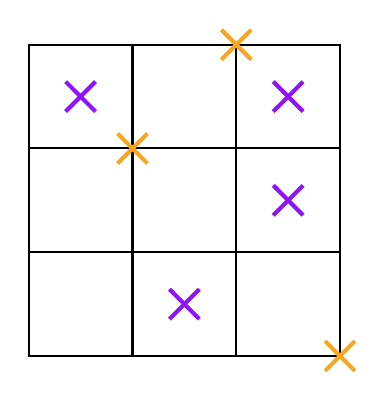
\begin{tikzpicture}[x=0.75pt,y=0.75pt,yscale=-1,xscale=1]
%uncomment if require: \path (0,300); %set diagram left start at 0, and has height of 300

%Shape: Square [id:dp4570817602982631] 
\draw   (100,29) -- (150,29) -- (150,79) -- (100,79) -- cycle ;
%Shape: Square [id:dp2903299358971252] 
\draw   (150,29) -- (200,29) -- (200,79) -- (150,79) -- cycle ;
%Shape: Square [id:dp8410481858286352] 
\draw   (100,79) -- (150,79) -- (150,129) -- (100,129) -- cycle ;
%Shape: Square [id:dp1117017430126368] 
\draw   (150,79) -- (200,79) -- (200,129) -- (150,129) -- cycle ;
%Shape: Square [id:dp9054195019818092] 
\draw   (200,29) -- (250,29) -- (250,79) -- (200,79) -- cycle ;
%Shape: Square [id:dp9918567360750739] 
\draw   (200,79) -- (250,79) -- (250,129) -- (200,129) -- cycle ;
%Shape: Square [id:dp6694249449139529] 
\draw   (100,129) -- (150,129) -- (150,179) -- (100,179) -- cycle ;
%Shape: Square [id:dp6467857772283392] 
\draw   (150,129) -- (200,129) -- (200,179) -- (150,179) -- cycle ;
%Shape: Square [id:dp32240121043282777] 
\draw   (200,129) -- (250,129) -- (250,179) -- (200,179) -- cycle ;
%Straight Lines [id:da5972676544083908] 
\draw [color={rgb, 255:red, 245; green, 166; blue, 35 }  ,draw opacity=1 ][line width=1.5]    (150,79) ;
\draw [shift={(150,79)}, rotate = 45] [color={rgb, 255:red, 245; green, 166; blue, 35 }  ,draw opacity=1 ][line width=1.5]    (-10.17,0) -- (10.17,0)(0,10.17) -- (0,-10.17)   ;
%Straight Lines [id:da06771970628563428] 
\draw [color={rgb, 255:red, 245; green, 166; blue, 35 }  ,draw opacity=1 ][line width=1.5]    (250,179) ;
\draw [shift={(250,179)}, rotate = 45] [color={rgb, 255:red, 245; green, 166; blue, 35 }  ,draw opacity=1 ][line width=1.5]    (-10.17,0) -- (10.17,0)(0,10.17) -- (0,-10.17)   ;
%Straight Lines [id:da1804222983474455] 
\draw [color={rgb, 255:red, 245; green, 166; blue, 35 }  ,draw opacity=1 ][line width=1.5]    (200,29) ;
\draw [shift={(200,29)}, rotate = 45] [color={rgb, 255:red, 245; green, 166; blue, 35 }  ,draw opacity=1 ][line width=1.5]    (-10.17,0) -- (10.17,0)(0,10.17) -- (0,-10.17)   ;
%Straight Lines [id:da7901030413597554] 
\draw [color={rgb, 255:red, 144; green, 19; blue, 254 }  ,draw opacity=1 ][line width=1.5]    (175,154) ;
\draw [shift={(175,154)}, rotate = 45] [color={rgb, 255:red, 144; green, 19; blue, 254 }  ,draw opacity=1 ][line width=1.5]    (-10.17,0) -- (10.17,0)(0,10.17) -- (0,-10.17)   ;
%Straight Lines [id:da37933960521297805] 
\draw [color={rgb, 255:red, 144; green, 19; blue, 254 }  ,draw opacity=1 ][line width=1.5]    (225,104) ;
\draw [shift={(225,104)}, rotate = 45] [color={rgb, 255:red, 144; green, 19; blue, 254 }  ,draw opacity=1 ][line width=1.5]    (-10.17,0) -- (10.17,0)(0,10.17) -- (0,-10.17)   ;
%Straight Lines [id:da13742234427535593] 
\draw [color={rgb, 255:red, 144; green, 19; blue, 254 }  ,draw opacity=1 ][line width=1.5]    (125,54) ;
\draw [shift={(125,54)}, rotate = 45] [color={rgb, 255:red, 144; green, 19; blue, 254 }  ,draw opacity=1 ][line width=1.5]    (-10.17,0) -- (10.17,0)(0,10.17) -- (0,-10.17)   ;
%Straight Lines [id:da5163777331330268] 
\draw [color={rgb, 255:red, 144; green, 19; blue, 254 }  ,draw opacity=1 ][line width=1.5]    (225,54) ;
\draw [shift={(225,54)}, rotate = 45] [color={rgb, 255:red, 144; green, 19; blue, 254 }  ,draw opacity=1 ][line width=1.5]    (-10.17,0) -- (10.17,0)(0,10.17) -- (0,-10.17)   ;




\end{tikzpicture}
